\chapter{The provisioning of the infrastructure}

\section*{Introduction}
\noindent
The first sprint of this project focused on provisioning the necessary cloud resources and setting the connections between them. In this chapter, we will present how we customized the architecture to our needs and the challenges we faced during the process, and we will also showcase the features implemented in the terraform modules.

\section{Activities Completed}
\begin{itemize}
    \item \textbf{Azure account setup:} We created an Azure account using the student package offer.
    \item \textbf{Azure CLI installation:} We installed the Azure CLI to manage our Azure resources.
    \item \textbf{created the necessary modules:} For a better organization of our code, we separated the resources into modules: the web app module, the database module and the storage account module.
    \item \textbf{established the network configurations:} We provisioned the virtual network and the DNS zones for each module and added the necessary links.
    \item \textbf{set up the different workspaces:} We created different workspaces for each environment (dev, QA, prod) and set the default values for each environment.
    \item \textbf{tested the architecture:} We tested the architecture by deploying the provisioned resources and deploying a simple web application.
    \item \textbf{wrote the documentation:} We wrote the documentation explaining how to modify the different variables and how to use the different workspaces(I auto-generated the documentation for the modules to ensure consistency using terraform-docs).
\end{itemize}
\section{The modified architecture:}
the slight modification made to the original architecture consisted of the removal of the application gateway due to its high price so the user will just have to access the web app directly which is acceptable since we only have one web app.
\\ the new simplified architecture is shown in figure \ref{fig:new_arch}.

\begin{figure}[htpb]
    \centering
    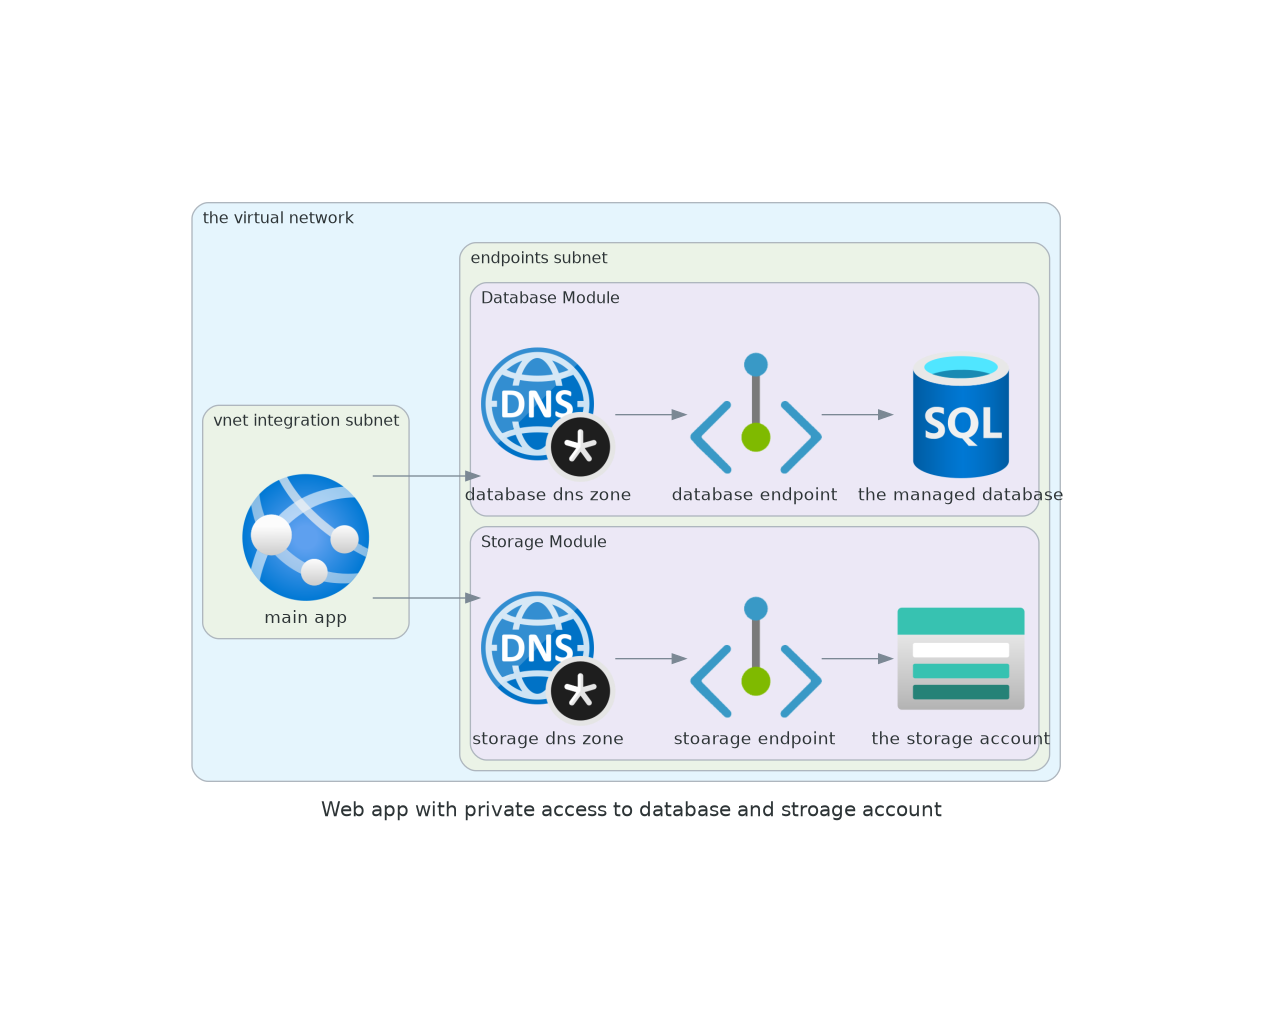
\includegraphics[width=0.8\textwidth]{web_app_with_private_access_to_database_and_stroage_account.png}
    \caption{The new architecture}
    \label{fig:new_arch}
\end{figure}

\section{Delivrables:}
the deliverables for this sprint are the terraform configuration that adapts to three different workspaces:
\begin{itemize}
    \item \textbf{dev:} the development environment:
    \begin{itemize}
        \item the resources are the most basic cost to optimize the cost.
        \item It also has a VM with a public IP inside the virtual network to access the database and the storage account.
        \item the web app and the VM can only be accessed from the CIDN given in the variables.
    \end{itemize}
    \item \textbf{QA:} the quality assurance environment:
    \begin{itemize}
        \item the resources are a bit more expensive to better simulate the production environment.
        \item It also has a VM with a public IP inside the virtual network to access the database and the storage account.
        \item it is open to the public.
    \end{itemize}
    \item \textbf{prod:} the production environment.
    \begin{itemize}
        \item the resources are the most expensive to ensure the best performance.
        \item it is open to the public.
    \end{itemize}
\end{itemize}
\subsection*{the file structure:}
this figure \ref{fig:file_structure} shows the file structure of the terraform configuration.

\begin{figure}[htpb]
    \centering
    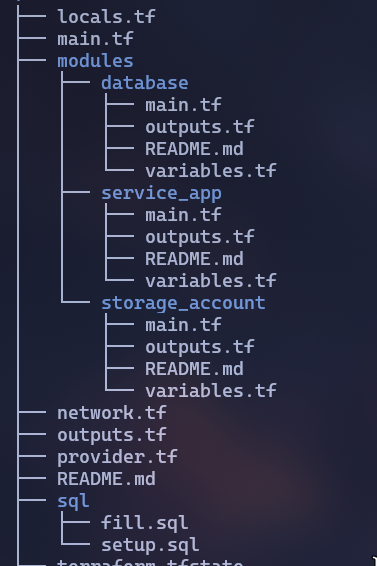
\includegraphics[width=0.3\textwidth]{file_structure.png}
    \caption{The file structure}
    \label{fig:file_structure}
\end{figure}
To promote code reusability, maintainability, and clarity, we adopted a modular approach for our Terraform configuration. This involved structuring the code into distinct modules, each encapsulating a specific aspect of the infrastructure (e.g., web app, database, storage account). This approach allows us to manage and update each module independently, and to reuse them across different environments.
\par
Furthermore, to ensure consistency and streamline configuration changes, we grouped frequently used variables like SKU names, VNet prefixes, and subnet prefixes into a dedicated local.tf file.
\par
This combined approach of modular structure and centralized variable management promotes efficient and well-organized Terraform configuration, fostering long-term project maintainability and scalability.
\section{Challenges:}
\subsection*{the problem:}
The main challenge we faced during Sprint 1 was configuring the DNS zones to enable communication between the web application and the database. Despite successfully provisioning the necessary cloud resources, the web application encountered issues resolving the hostname of the database. This meant the application couldn't locate the database to retrieve or store data, hindering core functionality. Troubleshooting involved verifying several aspects:

\begin{figure}[htpb]
    \centering
    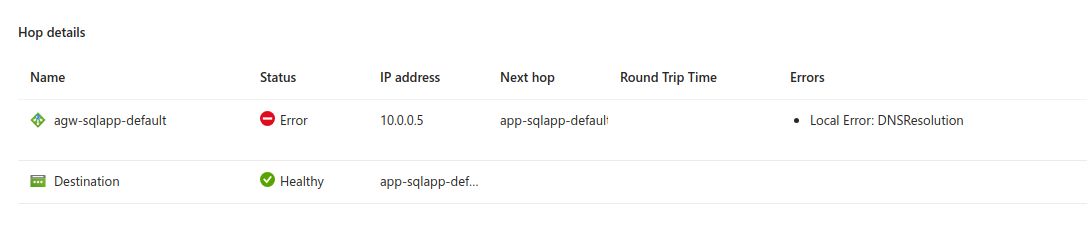
\includegraphics[width=0.8\textwidth]{connnectivity_problem.png}
    \caption{connnectivity problem}
    \label{fig:connection_problem}
\end{figure}

\begin{itemize}
    \item \textbf{DNS record configuration:} We double-checked the DNS record types (likely A record) and their values (database hostname and IP address) within the configured DNS zone. Any typos or incorrect mappings could have caused resolution issues.
    \item \textbf{Network security group (NSG) rules:} We had to verify the NSG rules to ensure the web application could communicate with the database.
    \item \textbf{verify connections:} We had to verify that the database was accessible from the web application. and that the web could access the DNS server.
\end{itemize}
By systematically examining these potential causes, we were able to identify that the web app did not have access to the DNS server provided by Azure. This experience highlights the importance of careful configuration and understanding of how DNS plays a crucial role in enabling communication between different components within a cloud infrastructure.
\subsection*{the solution:}
To address the DNS resolution issue between the web application and the database, we capitalized on a core Azure concept: \textbf{the Wire Server}. This managed DNS server, automatically created within each virtual network, plays a critical role in resolving internal DNS queries using private DNS zones. Although offered as a free service, the Wire Server isn't automatically configured as the default DNS server for the virtual network.

Our solution involved leveraging Terraform to explicitly set the Wire Server's static IP address (168.63.129.16) as the default DNS server within our virtual network configuration. By making this configuration change, we ensured that the web application could effectively utilize the Wire Server to resolve the database hostname and establish the necessary communication channel. This approach eliminated the initial DNS resolution obstacle and facilitated seamless communication between the application and the database.

\begin{figure}[htpb]
    \centering
    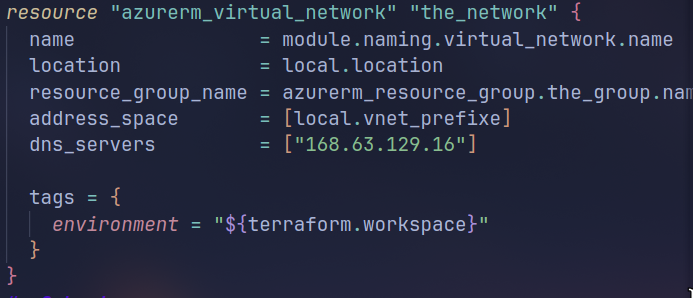
\includegraphics[width=0.8\textwidth]{DNS_server.png}
    \caption{The DNS configuration}
    \label{fig:dns_configuration}
\end{figure}

\section{Conclusion}
This chapter detailed the successful completion of Sprint 1, focusing on provisioning the cloud infrastructure for our project. We presented a modified architecture that removed the application gateway due to cost considerations. The new architecture leverages Terraform modules for efficient code organization and utilizes workspaces to manage different environments (dev, QA, prod) with appropriate resource configurations.
\par
We encountered a challenge during this sprint related to DNS configuration, where the web application struggled to resolve the database hostname. This issue was resolved by leveraging the Azure Wire Server as the default DNS server within the virtual network configuration.
\par
By successfully provisioning the infrastructure and addressing the DNS resolution challenge, Sprint 1 laid the foundation for future sprints to focus on building and deploying the web application and its functionalities.
